\documentclass[10pt,a4paper,twocolumn]{article}

\usepackage[utf8]{inputenc}
\usepackage[T1]{fontenc}
\usepackage{newtxtext,newtxmath}
\usepackage[margin=1.65cm]{geometry}
\usepackage{microtype}
\usepackage{graphicx}
\usepackage{booktabs}
\usepackage{tabularx}
\usepackage{array}
\usepackage{amsmath}
\usepackage{xcolor}
\usepackage{caption}
\usepackage{subcaption}
\usepackage{enumitem}
\usepackage{titlesec}
\usepackage{dblfloatfix}
\usepackage[section]{placeins}
\usepackage{balance}
\usepackage[hidelinks]{hyperref}
\usepackage{url}

\setlength{\columnsep}{0.62cm}
\setlength{\parindent}{1em}
\setlength{\parskip}{0pt}
\setlength{\emergencystretch}{1.5em}
\captionsetup{font=small,labelfont=bf}
\urlstyle{same}

\titleformat{\section}{\large\bfseries}{\thesection.}{0.45em}{}
\titleformat{\subsection}{\normalsize\bfseries}{\thesubsection.}{0.45em}{}

\newcommand{\ours}{\textbf{48.45\% $\pm$ 2.14\%}}
\newcommand{\paperavg}{49.60\%}

\title{\textbf{Acoustic-Only 1D CNN Baseline for Cross-Speed Electrical Motor Fault Diagnosis}\\
\large Contribution to the Workshop Project: \emph{Multimodal Deep Learning for Anomaly Detection of Electrical Motors Using Sound and Vibration Signals}}
\author{Apostolia Maria Sofianopoulou\\
\small Workshop Project, Polytechnic University of Tirana (UPT)}
\date{14 October 2026}

\begin{document}
\maketitle

\begin{abstract}
This report documents the acoustic-modality contribution to a workshop project on multimodal electrical-motor fault diagnosis. A paper-inspired one-dimensional convolutional neural network (1D CNN) was implemented in PyTorch and evaluated on the HUSTmotor multimodal dataset under the four leave-one-speed-out motor tasks defined by Zhao \emph{et al.} The upstream preprocessing was supplied by Gentian Qinami through the shared project repository and provides synchronized, z-score-normalized 1024-point acoustic and vibration windows with a block-based train/validation split. The acoustic baseline was trained for 50 epochs with Adam and evaluated over ten independent random seeds. Across Tasks 9--12, the implementation achieved an overall mean target accuracy of \ours, compared with \paperavg\ for the acoustic-only M2 baseline reported in the reference paper. Although the averages are close, task-wise and class-wise analyses reveal substantial differences: performance is particularly weak for the unseen 5 Hz domain and substantially stronger than the paper baseline for the unseen 30 Hz domain. These results show that aggregate accuracy alone can hide strong operating-condition and class dependencies, and they motivate the later multimodal fusion stage of the project.
\end{abstract}

\section{Scope and Reference Methodology}

The broader workshop investigates fault diagnosis of electrical motors from synchronized vibration and acoustic measurements. Within this project, the present contribution focuses specifically on the \textbf{acoustic branch}: exploratory signal analysis, implementation of the acoustic-only baseline, cross-speed evaluation, and interpretation of the learned model's failure modes. Although the project title uses the term ``anomaly detection,'' the baseline studied here is a \textbf{supervised six-class classification problem} in which each 1024-point acoustic window is assigned to one of six motor health states.

The implementation is based on the motor experiments in Zhao \emph{et al.}~\cite{zhao2025}, where the acoustic-only empirical-risk-minimization model is denoted \textbf{M2}. The paper uses a shared 1D CNN feature extractor for vibration and acoustic data and evaluates domain generalization by training on three motor speeds and testing on a fourth unseen speed. The full paper proposes the Multimodal Unified Generalization and Translation Network (MUGTN); however, the objective of this contribution is deliberately narrower: establish a reproducible acoustic-only reference before multimodal fusion is introduced.

\section{Dataset and Preprocessing Interface}

\subsection{HUSTmotor motor-fault data}

The HUSTmotor motor dataset contains six health conditions: \textit{healthy}, \textit{bearing fault}, \textit{bowed rotor}, \textit{broken rotor bars}, \textit{rotor misalignment}, and \textit{voltage unbalance}. Measurements are available at four operating speeds: 5, 10, 20, and 30 Hz. Vibration and acoustic signals are synchronously sampled at 25.6 kHz~\cite{zhao2025,hustdataset}. The reference paper uses 1024-point samples and prepares 1000 samples per health state and operating condition, with an 800/200 train-test division~\cite{zhao2025}.

The team preprocessing pipeline was prepared by Gentian Qinami and distributed through the shared repository~\cite{gentirepo}. The delivered file \texttt{hustmotor\_1024.npz} contains 24,000 paired windows:
\[
6\ \text{classes}\times4\ \text{speeds}\times1000\ \text{windows}=24{,}000.
\]
Its metadata records \texttt{win=1024}, \texttt{norm=zscore}, \texttt{split=block}, and \texttt{fs=25600}. Each 1024-point window therefore represents
\[
\frac{1024}{25{,}600}=0.04\ \text{s}=40\ \text{ms}
\]
of acoustic data. The acoustic and vibration windows retain common sample indices so that the unimodal results can later feed the multimodal stage.

\subsection{Block-based split and task construction}

A methodological difference from the paper is important. The reference study states that 800 of the 1000 samples per condition are randomly selected for training and 200 for testing~\cite{zhao2025}. The shared preprocessing release instead uses an \textbf{acquisition-block-based split}. Five blocks are represented for each class-speed pair; four blocks contribute 800 windows and the held-out block contributes 200 windows. This choice reduces the risk that strongly related or overlapping windows from the same acquisition block are placed on both sides of the split.

For each leave-one-speed-out task, the three source domains contribute 14,400 training windows and 3,600 source-validation windows, whereas the unseen target contributes 1,200 held-out windows. No target-domain sample is used for training, hyperparameter selection, or checkpoint selection. Table~\ref{tab:tasks} summarizes the four tasks.

\begin{table}[!t]
\centering
\caption{Motor domain-generalization tasks.}
\label{tab:tasks}
\small
\begin{tabular}{c c c}
\toprule
\textbf{Task} & \textbf{Source speeds (Hz)} & \textbf{Target (Hz)}\\
\midrule
9  & 10, 20, 30 & 5\\
10 & 5, 20, 30  & 10\\
11 & 5, 10, 30  & 20\\
12 & 5, 10, 20  & 30\\
\bottomrule
\end{tabular}
\end{table}

\section{Acoustic Signal Exploration}

Before model training, the raw acoustic modality was examined in both the time and frequency domains to determine whether it contained fault-related information and how strongly it was affected by motor speed. Two comparisons were particularly useful.

Figure~\ref{fig:eda-speed} fixes the bearing-fault condition and compares its acoustic spectrum at the four operating speeds. The spectral magnitude and structure vary substantially as speed changes, especially in the low-frequency region. This provides direct qualitative evidence that operating speed acts as a domain variable for the acoustic modality.

\begin{figure}[!t]
\centering
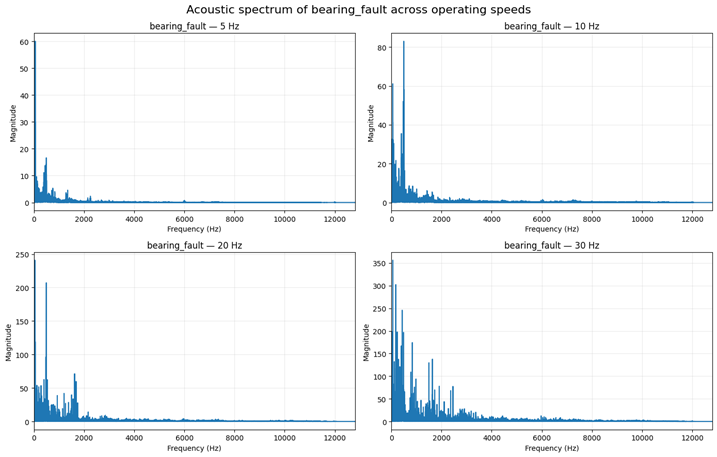
\includegraphics[width=\columnwidth]{figures/eda_speed.png}
\caption{Acoustic FFT of the bearing-fault condition across 5, 10, 20, and 30 Hz. The change in spectrum with speed motivates cross-domain evaluation.}
\label{fig:eda-speed}
\end{figure}

Figure~\ref{fig:eda-faults} instead fixes the operating speed at 20 Hz and compares the six health states. Distinct low-frequency spectral patterns are visible across classes, indicating that the acoustic signal contains discriminative fault information in addition to speed-dependent structure. Together, the two observations motivate a model that must learn fault-related representations while remaining robust to changes in operating condition.

\begin{figure}[!t]
\centering
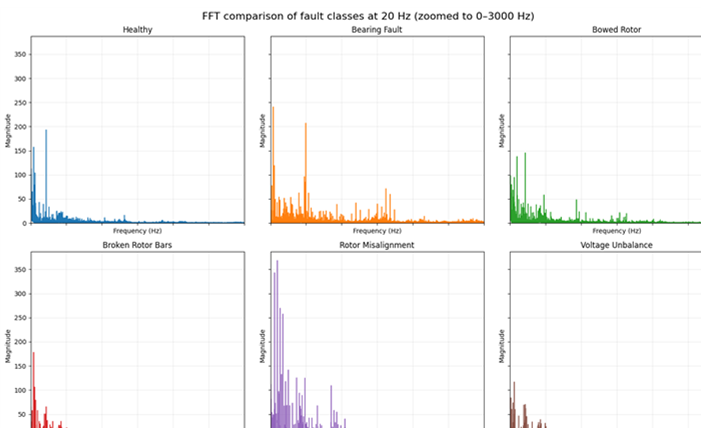
\includegraphics[width=\columnwidth]{figures/eda_faults.png}
\caption{FFT comparison of the six motor states at 20 Hz, zoomed to the 0--3000 Hz region. Fault-related differences remain visible when operating speed is fixed.}
\label{fig:eda-faults}
\end{figure}

\section{Implementation}

\subsection{Software stack and notebook organization}

The complete baseline was implemented in a public-facing Google Colab workflow. PyTorch is used for tensor operations, model definition, CUDA execution, optimization, and data loading. NumPy is used for loading the \texttt{.npz} archive and array-level checks; pandas stores epoch histories and aggregate results; scikit-learn provides confusion matrices and precision/recall/F1 metrics; and Matplotlib produces diagnostic figures. The setup code also uses \texttt{requests}, \texttt{tqdm}, and \texttt{hashlib} to download the preprocessing release, display progress, and verify the dataset SHA-256 fingerprint before training.

The notebook automatically selects a CUDA device when available and otherwise falls back to CPU execution. PyTorch \texttt{DataLoader} objects feed mini-batches of 256 samples. Acoustic arrays arrive with shape $(N,1024)$ and are converted to $(N,1,1024)$ because \texttt{Conv1d} expects the ordering \texttt{(batch, channels, length)}. Class labels are converted to 64-bit integer tensors as required by cross-entropy loss.

Reproducibility is handled by seeding Python, NumPy, and PyTorch. Deterministic cuDNN behavior is requested, and ten independent seeds (0--9) are used for the final benchmark. The dataset file is hash-verified before use, and all model checkpoints and tabular results are stored separately from the notebook runtime.

\subsection{Paper-inspired 1D CNN}

The reference paper specifies four convolution/max-pooling blocks for the feature extractor $F_a$, with 16, 32, 64, and 64 filters and kernel sizes 64, 16, 5, and 5 respectively~\cite{zhao2025}. Each convolution uses stride 1 and is associated with ReLU activation and batch normalization; max-pooling uses kernel size 2 and stride 2. The state classifier is a fully connected layer followed conceptually by Softmax~\cite{zhao2025}.

Table~\ref{tab:architecture} gives the exact PyTorch realization used here. Because the paper does not explicitly state the convolution padding, this implementation uses \textbf{valid convolution} (\texttt{padding=0}). Likewise, the code adopts the common sequence \texttt{Conv1D $\rightarrow$ BatchNorm $\rightarrow$ ReLU $\rightarrow$ MaxPool}. These are explicit reproduction assumptions rather than details claimed to be specified by the paper.

\begin{table*}[!t]
\centering
\caption{Acoustic 1D CNN architecture implemented in PyTorch. Output lengths assume \texttt{padding=0}.}
\label{tab:architecture}
\small
\begin{tabular}{l c c c c c}
\toprule
\textbf{Stage} & \textbf{Input channels} & \textbf{Output channels} & \textbf{Kernel / stride} & \textbf{Output length} & \textbf{Operation}\\
\midrule
Input & 1 & 1 & -- & 1024 & z-score-normalized acoustic window\\
Conv block 1 & 1 & 16 & $64/1$ & $961\rightarrow480$ & Conv1D + BN + ReLU + MaxPool$(2)$\\
Conv block 2 & 16 & 32 & $16/1$ & $465\rightarrow232$ & Conv1D + BN + ReLU + MaxPool$(2)$\\
Conv block 3 & 32 & 64 & $5/1$ & $228\rightarrow114$ & Conv1D + BN + ReLU + MaxPool$(2)$\\
Conv block 4 & 64 & 64 & $5/1$ & $110\rightarrow55$ & Conv1D + BN + ReLU + MaxPool$(2)$\\
Flatten & 64 & -- & -- & $64\times55=3520$ & feature vector\\
Classifier & -- & 6 & -- & 6 & fully connected logits\\
\bottomrule
\end{tabular}
\end{table*}

The final convolutional tensor has shape $(64,55)$ per sample. Flattening therefore produces $64\times55=3520$ learned acoustic features, which are passed to a $3520\rightarrow6$ linear classifier. The model contains approximately 61,590 trainable parameters. The feature vector is exposed separately in the implementation so that it can later be reused by the multimodal fusion branch.

The paper lists a Softmax output, but no explicit Softmax layer is placed inside the PyTorch \texttt{forward()} function during training. Instead, the network returns raw logits and uses \texttt{CrossEntropyLoss}, which internally performs the numerically stable log-Softmax operation required for multiclass cross entropy. Softmax is therefore only needed when calibrated class probabilities are explicitly requested; the predicted class is obtained by \texttt{argmax} on the logits.

\section{Training and Evaluation Protocol}

Training follows the reference settings where they are explicitly available. Adam is used for optimization, the batch size is 256, and each model is trained for 50 epochs~\cite{zhao2025}. The epoch-dependent learning rate is
\begin{equation}
\mathrm{lr}(\phi)=\frac{0.0005}{(1+10\phi)^{0.75}},
\end{equation}
where $\phi$ is the ratio of the current epoch to the total number of epochs. The paper averages diagnostic results over ten independent trials, which is reproduced here with ten random seeds~\cite{zhao2025}.

An additional implementation decision is checkpoint selection. After each epoch, the model is evaluated on the source-domain validation split. The checkpoint with the highest source-validation accuracy is retained and restored at the end of training. The unseen target set is then evaluated only after model selection has finished. This separates model selection from the domain-generalization test and prevents target leakage.

For each task, the final evaluation records target accuracy, per-class precision, recall and F1-score, and a row-normalized confusion matrix. Ten trained checkpoints are evaluated and aggregated to obtain mean and standard deviation. The single-seed learning behavior in Fig.~\ref{fig:learning} is representative of the optimization dynamics: training accuracy approaches 100\%, while source-validation accuracy stabilizes near the low 90s. The substantial gap between source validation and unseen-target performance in some tasks therefore reflects cross-domain generalization difficulty rather than failure to fit the source data.

\begin{figure}[!t]
\centering
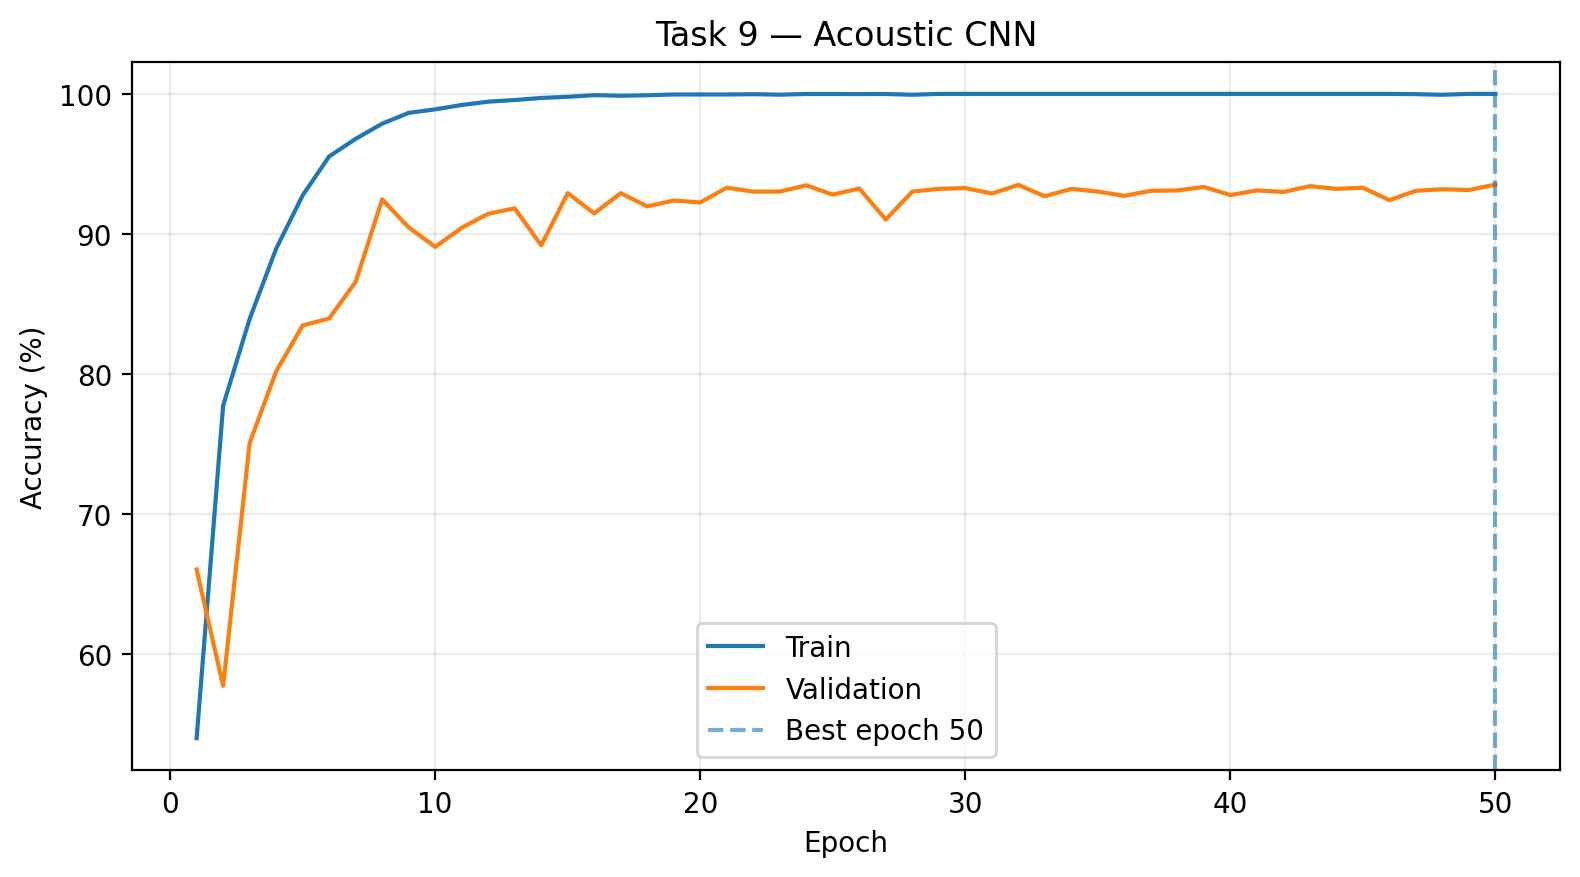
\includegraphics[width=\columnwidth]{figures/task9_learning_curve.png}
\caption{Task 9 learning curve for seed 0. The selected checkpoint is based only on source-domain validation accuracy; the unseen 5 Hz target is not used during training or selection.}
\label{fig:learning}
\end{figure}

\section{Results}

\subsection{Task-level accuracy}

Table~\ref{tab:results} compares the ten-run acoustic results with the paper's M2 baseline. The overall mean across Tasks 9--12 is \ours, only 1.15 percentage points below the paper's reported 49.60\%. Nevertheless, the close average should not be interpreted as an exact reproduction because the individual task behavior differs substantially.

\begin{table*}[!t]
\centering
\caption{Ten-run acoustic-only target accuracy compared with the reference paper. ``Difference'' is our mean minus the paper M2 value.}
\label{tab:results}
\small
\begin{tabular}{c c c c c c}
\toprule
\textbf{Task} & \textbf{Source speeds (Hz)} & \textbf{Target} & \textbf{Our accuracy (\%)} & \textbf{Paper M2 (\%)} & \textbf{Difference (pp)}\\
\midrule
9  & 10, 20, 30 & 5 Hz  & $26.36\pm2.997$ & $49.23\pm4.71$ & $-22.87$\\
10 & 5, 20, 30  & 10 Hz & $60.96\pm4.024$ & $61.89\pm2.57$ & $-0.93$\\
11 & 5, 10, 30  & 20 Hz & $57.29\pm4.878$ & $59.14\pm1.05$ & $-1.85$\\
12 & 5, 10, 20  & 30 Hz & $49.19\pm2.803$ & $28.13\pm1.77$ & $+21.06$\\
\midrule
\multicolumn{3}{r}{\textbf{Average}} & \textbf{48.45} & \textbf{49.60} & \textbf{$-1.15$}\\
\bottomrule
\end{tabular}
\end{table*}

Tasks 10 and 11 are numerically close to the reference results. Task 9 is substantially more difficult in the present implementation, with only $26.36\%\pm3.00\%$ accuracy on unseen 5 Hz data. In contrast, Task 12 reaches $49.19\%\pm2.80\%$, exceeding the paper's M2 value by approximately 21 percentage points. Figure~\ref{fig:comparison} makes this cancellation effect visible: a poor Task 9 result and a strong Task 12 result produce an average that happens to be close to the paper baseline.

\begin{figure*}[!t]
\centering
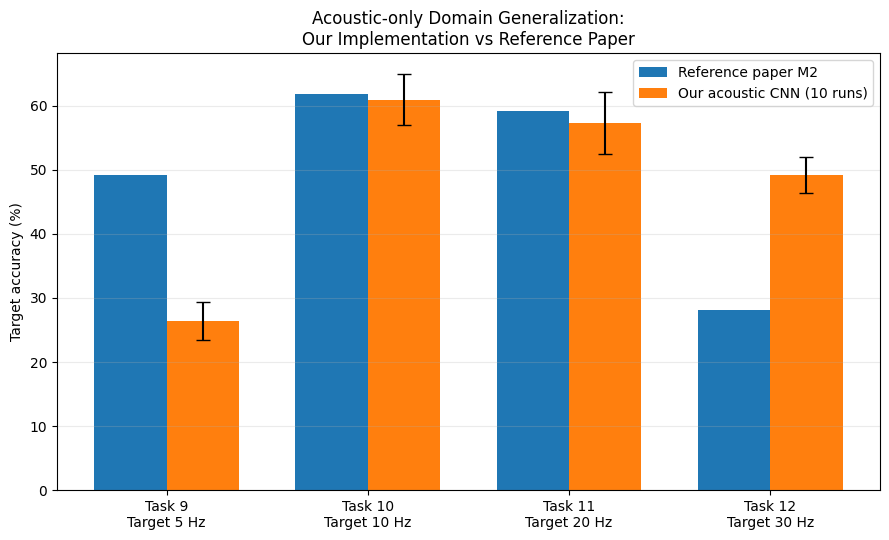
\includegraphics[width=0.78\textwidth]{figures/paper_vs_ours.png}
\caption{Our ten-run acoustic-only accuracy versus the reference M2 values. Error bars show one standard deviation across the ten trained models.}
\label{fig:comparison}
\end{figure*}

The mean source-validation accuracies across the same ten runs were 91.24\%, 89.76\%, 87.02\%, and 88.76\% for Tasks 9--12 respectively. Thus, the particularly low Task 9 target accuracy is not explained by inability to classify the source domains; it is associated with a severe shift between the learned source distribution and the unseen 5 Hz condition.

\subsection{Class-wise behavior}

Aggregate row-normalized confusion matrices are shown in Fig.~\ref{fig:cms}. Each cell is averaged over ten independently trained models. The class-wise analysis reveals that the effect of speed shift is strongly non-uniform.

\begin{figure*}[!t]
\centering
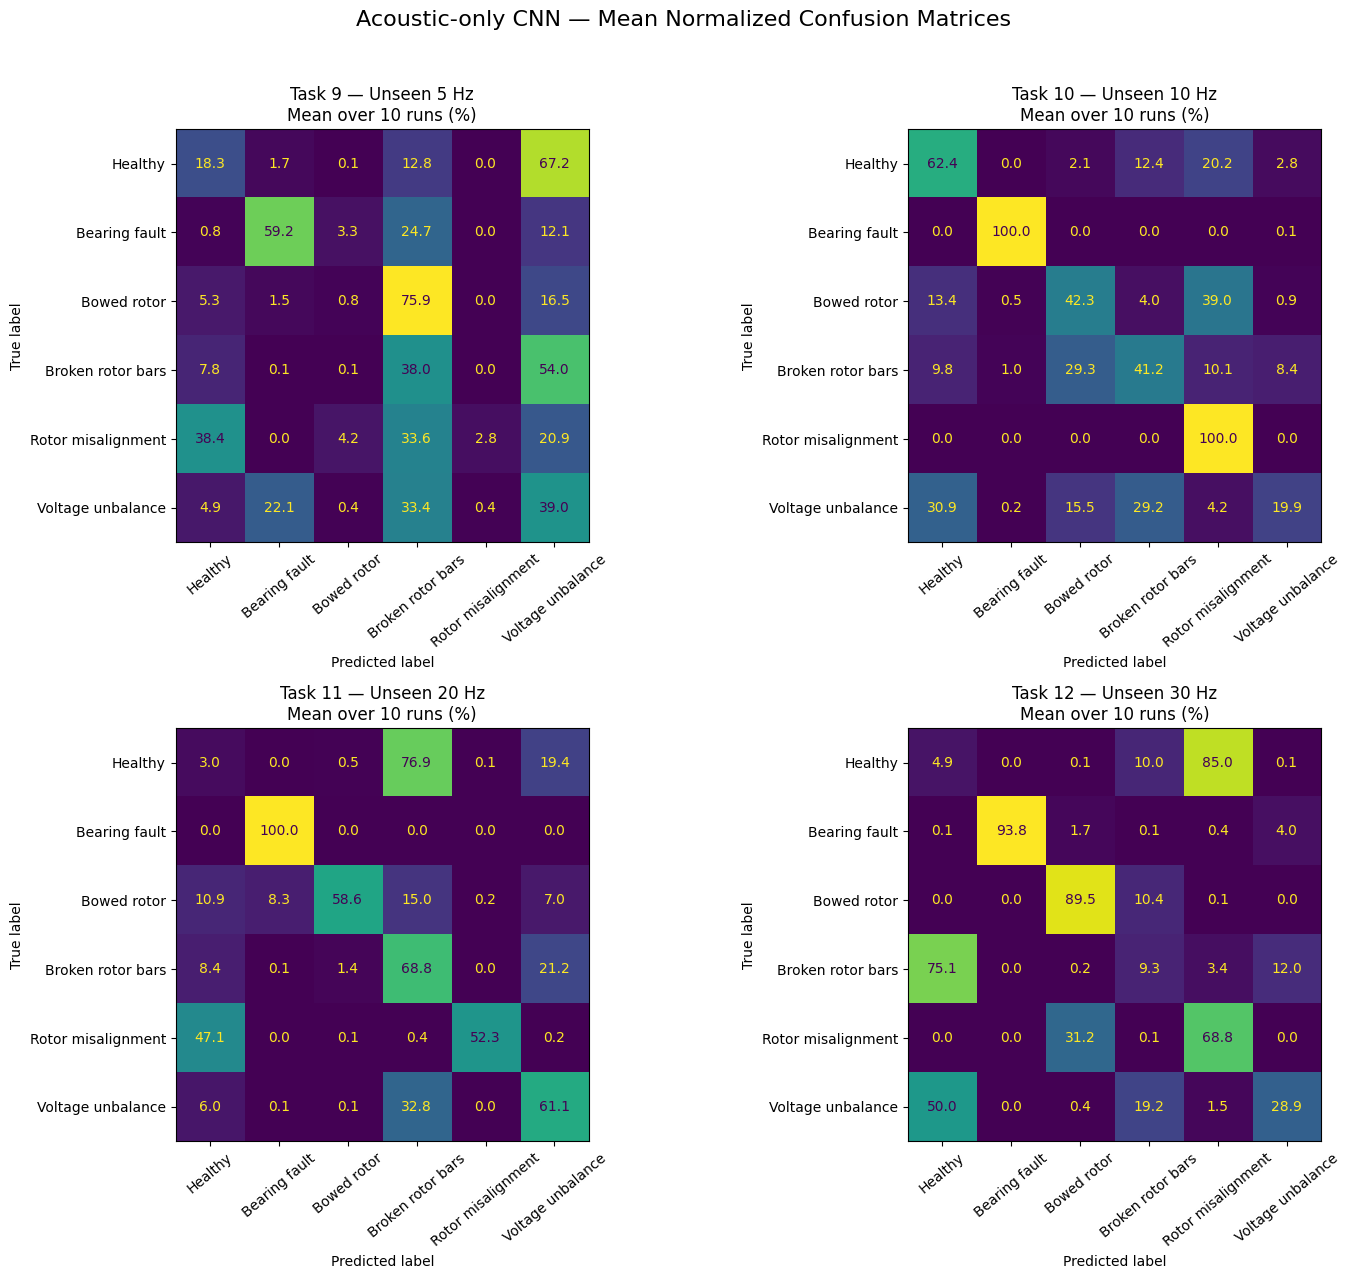
\includegraphics[width=0.97\textwidth]{figures/aggregate_confusions.png}
\caption{Mean row-normalized confusion matrices for Tasks 9--12 over ten independent runs. Rows are true classes and columns are predicted classes; values are percentages.}
\label{fig:cms}
\end{figure*}

For Task 9, bearing fault retains moderate recall (59.15\%), while bowed rotor (0.85\%), rotor misalignment (2.85\%), and healthy (18.30\%) transfer very poorly to 5 Hz. Healthy samples are predominantly predicted as voltage unbalance, and bowed-rotor samples are predominantly mapped to broken rotor bars. The resulting macro-F1 is only 23.28\%.

Task 10 is considerably more stable. Bearing fault reaches 99.95\% recall and rotor misalignment reaches 100\% recall. However, the rotor-misalignment precision is only 57.90\%, showing that perfect recall does not imply balanced classification; samples from other classes are also attracted to that label. The Task 10 macro-F1 is 57.83\%.

For Task 11, bearing fault again reaches 100\% recall and several fault classes transfer reasonably well, but healthy samples collapse almost completely: healthy recall is only 3.05\%, with most of those samples predicted as broken rotor bars. The macro-F1 is 57.45\%.

Task 12 provides another instructive example. Bearing fault and bowed rotor achieve 93.80\% and 89.55\% recall respectively, and rotor misalignment reaches 68.75\%. At the same time, healthy and broken rotor bars achieve only 4.85\% and 9.30\% recall. The overall improvement over the paper's Task 12 accuracy therefore does not mean that all six classes generalize well; rather, strong transfer for some faults compensates for severe failure in others. The Task 12 macro-F1 is 47.72\%.

\begin{table}[!t]
\centering
\caption{Macro-F1 obtained from the ten-run class-wise analysis.}
\label{tab:macrof1}
\small
\begin{tabular}{c c c}
\toprule
\textbf{Task} & \textbf{Target speed} & \textbf{Macro-F1 (\%)}\\
\midrule
9 & 5 Hz  & 23.28\\
10 & 10 Hz & 57.83\\
11 & 20 Hz & 57.45\\
12 & 30 Hz & 47.72\\
\bottomrule
\end{tabular}
\end{table}

\section{Discussion}

The results support three main conclusions. First, the acoustic modality is clearly capable of fault discrimination, as shown both by the fixed-speed spectral analysis and by the relatively high performance on Tasks 10 and 11. Second, acoustic features are strongly dependent on operating speed. The dramatic degradation in Task 9, despite source-validation accuracy above 90\%, is direct evidence that source-domain classification quality does not guarantee unseen-speed robustness. Third, aggregate accuracy can be misleading: the overall value of 48.45\% is close to the paper's 49.60\%, yet the task-level behavior is markedly different.

Several methodological differences may contribute to the discrepancy and should be treated as limitations rather than hidden. The most important is the preprocessing split: the reference paper describes a random 800/200 partition, whereas the shared project release uses acquisition blocks to reduce overlap leakage. In addition, the paper does not explicitly specify convolution padding or the exact BatchNorm/ReLU ordering. The present implementation therefore documents its use of valid convolution and Conv--BatchNorm--ReLU ordering. Finally, checkpoint selection using a dedicated source-validation set is an explicit implementation decision intended to preserve the unseen target as a genuine final test.

These points mean that the present experiment should be described as a \textbf{paper-inspired reproduction of the M2 acoustic baseline}, not as a bit-for-bit reproduction of the authors' original code. The numerical agreement on the global average is encouraging, but the stronger scientific finding is the task- and class-specific sensitivity exposed by the ten-run analysis.

From the perspective of the full multimodal project, these weaknesses are useful rather than merely negative. Different classes fail under different speeds, suggesting that a second modality may provide complementary evidence exactly where the acoustic representation is unstable. The learned 3520-dimensional acoustic feature vector is therefore retained as an interface for later feature-level or more advanced multimodal fusion with the vibration branch.

\section{Conclusion}

A complete acoustic-only 1D CNN baseline was implemented and evaluated under the four HUSTmotor leave-one-speed-out tasks. The workflow integrates the team's shared preprocessing, a paper-inspired CNN architecture, leakage-aware source/target separation, deterministic training controls, checkpoint selection on source validation data, and ten-seed aggregate evaluation. The final overall target accuracy is \ours\ compared with \paperavg\ in the reference paper, but detailed analysis reveals large operating-condition and class-dependent differences. In particular, unseen 5 Hz data remain challenging, while the 30 Hz task substantially exceeds the reference M2 result. These findings establish a reproducible acoustic baseline and provide a clear motivation for the next project stage: combining acoustic and vibration representations to improve robustness across operating conditions.

\FloatBarrier
\balance
\begin{thebibliography}{9}

\bibitem{zhao2025}
C. Zhao, W. Shen, E. Zio, and H. Ma,
``Multimodal unified generalization and translation network for intelligent fault diagnosis under dynamic environments,''
\emph{Engineering Applications of Artificial Intelligence}, vol. 162, Art. no. 112559, 2025.
\href{https://doi.org/10.1016/j.engappai.2025.112559}{doi:10.1016/j.engappai.2025.112559}.

\bibitem{hustdataset}
C. Zhao \emph{et al.},
``HUSTmotor Multi-Modal Dataset,'' GitHub repository.
\url{https://github.com/CHAOZHAO-1/HUSTmotor-multi-modal-dataset}.

\bibitem{gentirepo}
G. Qinami,
``ISCF Project -- HUSTmotor preprocessing and domain-generalization data preparation,'' GitHub repository.
\url{https://github.com/Genti24-bit/ISCF_Project/}.

\end{thebibliography}

\end{document}
